% !TEX program = xelatex
\documentclass[11pt, a4paper]{article}
\usepackage{tikz}
\usetikzlibrary{calc, positioning}

\begin{document}

\section{Calc Library: Coordinate Calculations}

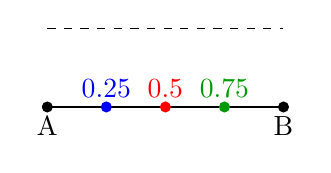
\begin{tikzpicture}
  \coordinate (A) at (0,0);
  \coordinate (B) at (3,0);

  % Draw the line from A to B
  \draw[thick] (A) -- (B);

  % Mark points A and B
  \fill (A) circle (2pt) node[below] {A};
  \fill (B) circle (2pt) node[below] {B};

  % Midpoint (0.5)
  \fill[red] ($(A)!0.5!(B)$) circle (2pt) node[above] {0.5};

  % Quarter point (0.25)
  \fill[blue] ($(A)!0.25!(B)$) circle (2pt) node[above] {0.25};

  % Three-quarters point (0.75)
  \fill[green!60!black] ($(A)!0.75!(B)$) circle (2pt) node[above] {0.75};

  % Vertical offset line
  \draw[dashed] ($(A) + (0,1)$) -- ($(B) + (0,1)$);
\end{tikzpicture}

\end{document}
